\documentclass[a4paper,11pt]{article}

\usepackage[margin=2.5cm]{geometry}
\usepackage[T1]{fontenc}
\usepackage[utf8]{inputenc}
\usepackage[english]{babel}
\usepackage{lmodern}
\usepackage{microtype}
\usepackage{amsmath}
\usepackage{booktabs}
\usepackage{tabularx}
\usepackage{float}
\usepackage{graphicx}
\usepackage{hyperref}
\usepackage{xcolor}

\hypersetup{
  colorlinks=true,
  linkcolor=blue!50!black,
  urlcolor=blue!50!black,
  pdftitle={IoT Challenge 3 -- Part 1 (Challenge)},
  pdfauthor={Tommaso Neri}
}

\setlength{\parindent}{0pt}
\setlength{\parskip}{0.55em}
\renewcommand{\arraystretch}{1.18}
\linespread{1.04}

\newcommand{\coursename}{Internet of Things Lab}
\newcommand{\challengename}{IoT Challenge \#3 -- Part 1 (Challenge)}
\newcommand{\authorname}{Tommaso Neri}
\newcommand{\personcode}{10817232}
\newcommand{\groupinfo}{Individual submission}
\newcommand{\todoanswer}[1]{\textbf{\textcolor{red}{#1}}}

\newcommand{\maybeincludegraphics}[3]{
  \IfFileExists{#1}{
    \includegraphics[#2]{#1}
  }{
    \fbox{
      \begin{minipage}[c][0.18\textheight][c]{0.88\linewidth}
        \centering
        \textbf{Missing figure:} #1\\
        #3
      \end{minipage}
    }
  }
}

\title{\challengename}
\author{
  \authorname\\
  Person Code: \personcode\\
  \groupinfo
}
\date{\today}

\begin{document}

\maketitle
\thispagestyle{empty}

\section*{Overview}

The implemented Node-RED flow processes the dataset \texttt{challenge3.csv}
using the MQTT-based identifier generator required by the assignment. The flow
uses a local Mosquitto broker on \texttt{localhost:1884}, publishes and
subscribes to the topic \texttt{challenge3/id\_generator}, extracts the CSV row
identified by:
\[
  N = ID \bmod 5218,
\]
and handles the two required packet classes:

\begin{itemize}
    \item packets whose \texttt{Command String} contains a \texttt{ZBEE\_ZCL}
    layer;
    \item packets whose \texttt{Packet Type} is \texttt{Link Status (0x08)}.
\end{itemize}

All other packets are ignored, but they still count toward the limit of 200
received ID messages. The processing stop condition is implemented in the
subscriber branch. The generator is also stopped automatically after the
subscriber completes the 200 received IDs, in order to avoid producing an
oversized \texttt{id\_log.csv}.

\section*{Node-RED Flow}

\begin{figure}[H]
\centering
\maybeincludegraphics{figures/node_red_flow.png}{width=\linewidth}{Insert here the screenshot of the complete Node-RED flow.}
\caption{Complete Node-RED flow used for Challenge 3.}
\end{figure}

The flow is organized into six main blocks, matching the structure of the
assignment: initialization, ID generation, ID subscription and CSV selection,
ZBEE\_ZCL publishing and filtered attributes, Link Status processing, and
ThingSpeak updates.

\section*{Initialization}

The \texttt{Init/reset files} inject node triggers the function
\texttt{reset counters + CSV headers}. This function resets all flow variables
used during the execution:

\begin{itemize}
    \item \texttt{id\_log\_no}, used as row counter for \texttt{id\_log.csv};
    \item \texttt{id\_rx\_count}, used to enforce the 200 received ID limit;
    \item \texttt{filtered\_no}, used as row counter for
    \texttt{filtered\_elems.csv};
    \item \texttt{link\_costs} and \texttt{link\_order}, used to store final
    Link Status costs while preserving processing order;
    \item \texttt{challenge\_done}, used to stop processing after 200 received
    IDs;
    \item \texttt{thingspeak\_started}, used to start the ThingSpeak branch only
    once;
    \item \texttt{generator\_enabled}, used to manually start or stop the ID
    generator.
\end{itemize}

The same function also rewrites the headers of the three output CSV files:
\texttt{id\_log.csv}, \texttt{filtered\_elems.csv}, and
\texttt{outgoing\_cost.csv}.

\section*{ID Generator Branch}

The ID generator is controlled by the \texttt{Start generator} and
\texttt{Stop generator} inject nodes. A periodic inject node named
\texttt{1s generator tick} fires once per second. The function
\texttt{generate MQTT ID + CSV row} checks whether generation is enabled and,
if so, creates:

\begin{itemize}
    \item a random ID in the range $[0, 30000]$;
    \item the current UNIX timestamp;
    \item the MQTT payload
    \texttt{\{"id": ID, "timestamp": TIMESTAMP\}};
    \item one row for \texttt{id\_log.csv}.
\end{itemize}

The MQTT message is published through the \texttt{mqtt out} node on:
\begin{center}
  \texttt{challenge3/id\_generator}.
\end{center}

The CSV row is appended to \texttt{id\_log.csv} with the required format:
\begin{center}
  \texttt{No.,ID,TIMESTAMP}.
\end{center}

\section*{Subscriber and CSV Selection Branch}

The \texttt{mqtt in} node subscribes to
\texttt{challenge3/id\_generator} on the local broker. The function
\texttt{count <=200 + N=id\%5218} parses the JSON payload, extracts the ID,
increments the subscriber-side counter, and computes:
\[
  N = ID \bmod 5218.
\]

When the received ID counter reaches 200, the flow variable
\texttt{challenge\_done} is set. Further messages are not processed.

The \texttt{file in} node reads \texttt{challenge3.csv}, and the \texttt{csv}
node parses it as an array of rows. The function
\texttt{select Packet Number N + classify} selects the row whose
\texttt{Packet Number} is equal to $N$ and routes the message as follows:

\begin{itemize}
    \item to the ZBEE\_ZCL branch if \texttt{Command String} contains
    \texttt{ZBEE\_ZCL};
    \item to the Link Status branch if \texttt{Packet Type} is
    \texttt{Link Status (0x08)};
    \item to a disabled debug node otherwise.
\end{itemize}

\section*{ZBEE\_ZCL Publish Branch}

For ZBEE\_ZCL packets, the function \texttt{prepare ZBEE\_ZCL MQTT payload}
builds the MQTT topic:
\begin{center}
  \texttt{ZigBee/<Device Name ZigBee Source>}.
\end{center}

The same topic is assigned both to \texttt{msg.topic} and to the \texttt{topic}
field inside the JSON payload, as required by the assignment clarification.

The published payload contains:

\begin{itemize}
    \item current UNIX timestamp;
    \item ID received by the subscription;
    \item WPAN source and destination addresses;
    \item ZigBee source and destination addresses;
    \item MQTT topic;
    \item original \texttt{Command String}.
\end{itemize}

The \texttt{delay} node named \texttt{rate limit 10/min queue} limits this
branch to 10 messages per minute. It is configured in queue mode, so messages
are delayed but not dropped. The rate-limited messages are sent to the local
MQTT broker through the \texttt{publish ZigBee/<device>} node.

\section*{Filtered Attributes and Dashboard Charts}

After the ZBEE\_ZCL rate limiter, the function \texttt{parse filtered attrs}
parses the command string and searches for the required attributes:

\begin{itemize}
    \item \texttt{Active Power};
    \item \texttt{RMS Current};
    \item \texttt{RMS Voltage}.
\end{itemize}

The function keeps the positional association required by the assignment:
\begin{center}
  \texttt{Attribute[i]} $\leftrightarrow$
  \texttt{Status[i]} $\leftrightarrow$
  \texttt{Data Type[i]} $\leftrightarrow$
  \texttt{Data Value[i]}.
\end{center}

Only complete attributes are saved. If the corresponding status, data type, or
value is missing, that attribute is excluded and no empty CSV cell is written.

Valid rows are appended to \texttt{filtered\_elems.csv} with the required
format:
\begin{center}
  \texttt{No.,Timestamp,Sequence Number, Attribute,Status,Data Type,Data Value}.
\end{center}

The numeric values of \texttt{RMS Current} and \texttt{RMS Voltage} are also sent
to two Node-RED dashboard chart nodes. No custom timestamp is set for the chart:
the dashboard uses the time at which the message reaches the chart node.

\begin{figure}[H]
\centering
\maybeincludegraphics{figures/node_red_rms_current.png}{width=0.9\linewidth}{Insert here the Node-RED dashboard screenshot for RMS Current.}
\caption{Node-RED dashboard chart for RMS Current.}
\end{figure}

\begin{figure}[H]
\centering
\maybeincludegraphics{figures/node_red_rms_voltage.png}{width=0.9\linewidth}{Insert here the Node-RED dashboard screenshot for RMS Voltage.}
\caption{Node-RED dashboard chart for RMS Voltage.}
\end{figure}

For additional verification from the generated CSV files, the following plots
were produced from the final outputs:

\begin{figure}[H]
\centering
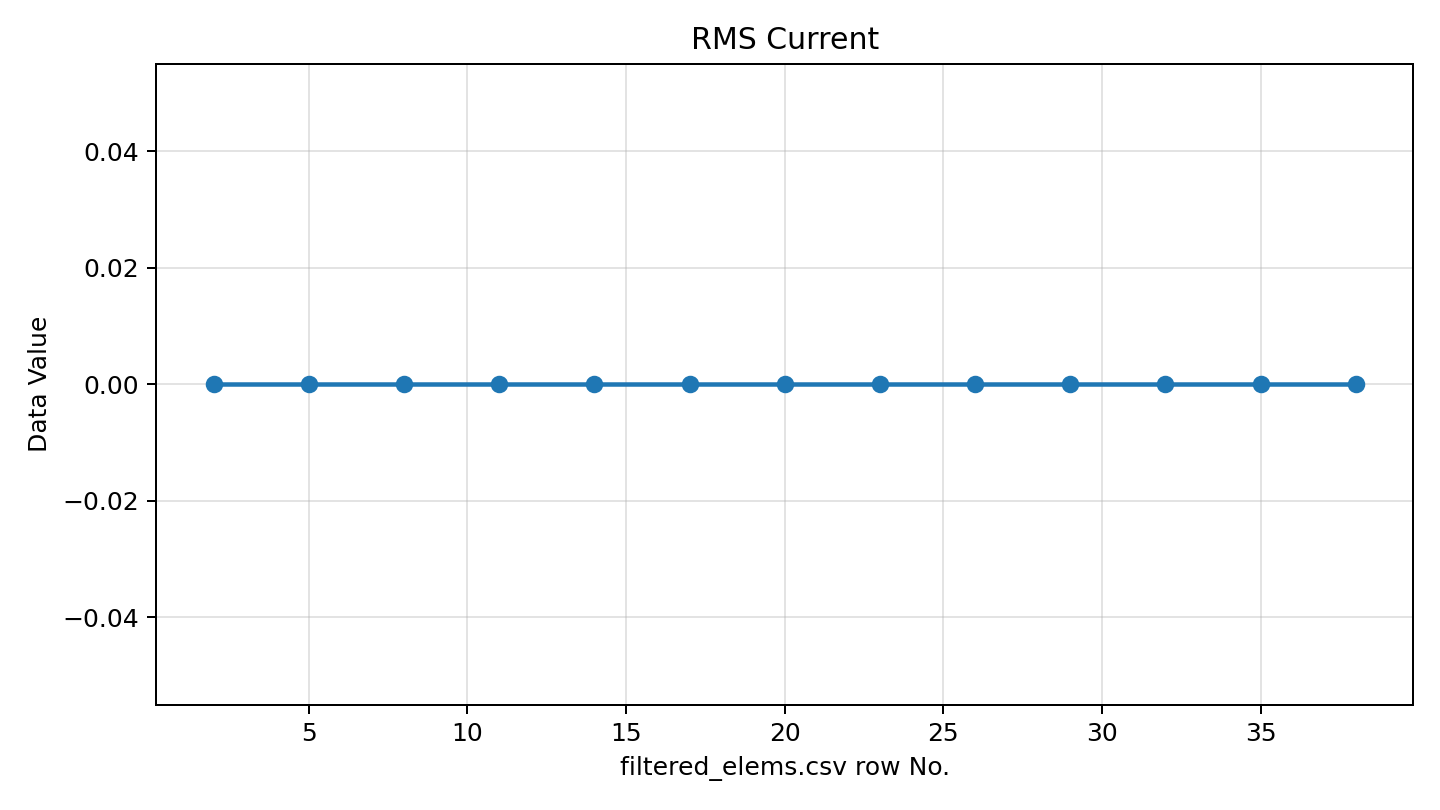
\includegraphics[width=0.82\linewidth]{report_assets/rms_current.png}
\caption{RMS Current values generated from \texttt{filtered\_elems.csv}.}
\end{figure}

\begin{figure}[H]
\centering
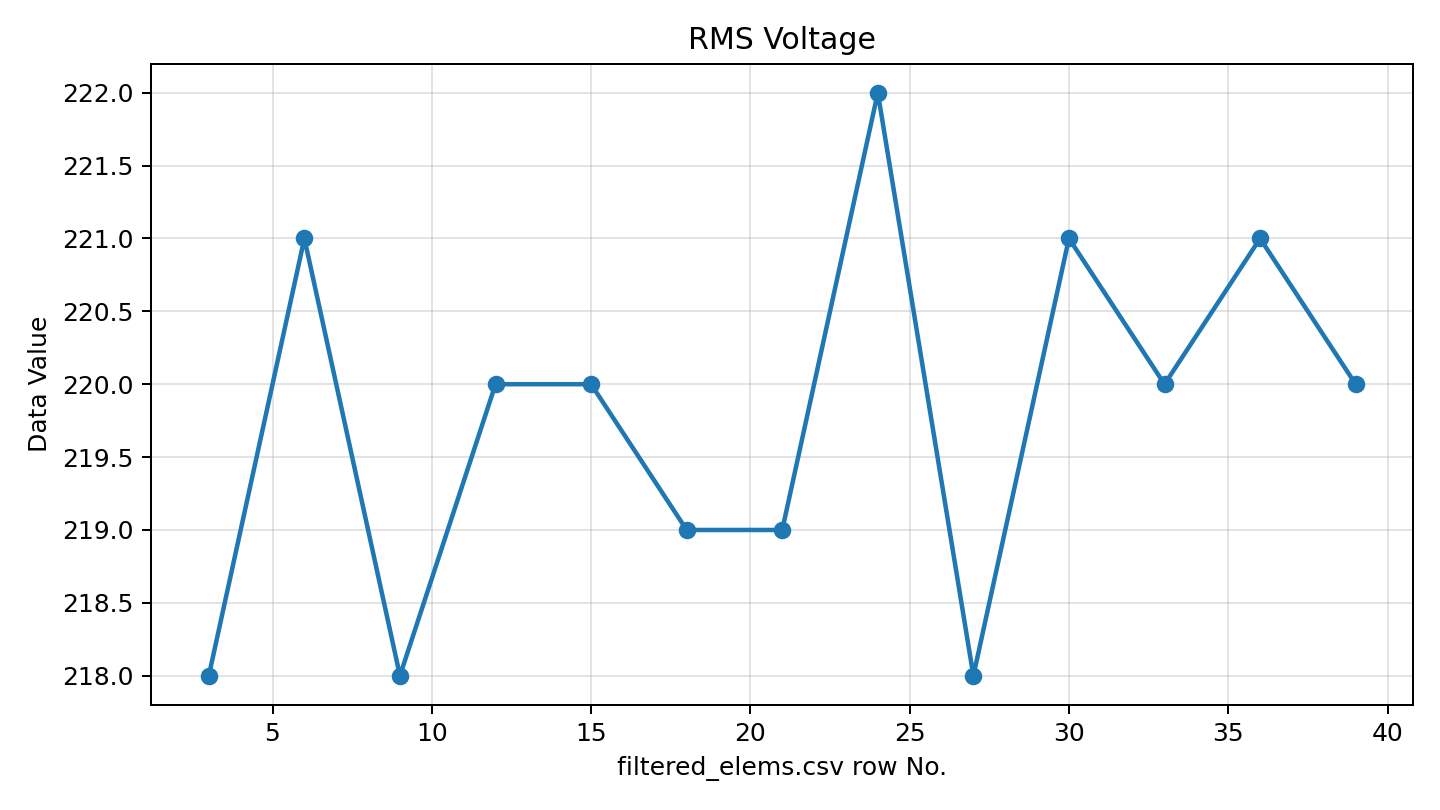
\includegraphics[width=0.82\linewidth]{report_assets/rms_voltage.png}
\caption{RMS Voltage values generated from \texttt{filtered\_elems.csv}.}
\end{figure}

\section*{Link Status Branch}

Packets are classified as Link Status packets by checking:
\begin{center}
  \texttt{Packet Type = Link Status (0x08)}.
\end{center}

The function \texttt{parse Link Status} parses the \texttt{Command String} and
extracts the list of links. For each link, it stores:

\begin{itemize}
    \item \texttt{Source}: the row value of \texttt{Source Address ZigBee};
    \item \texttt{Destination}: the link address;
    \item \texttt{Cost}: the link outgoing cost.
\end{itemize}

If a later Link Status packet updates an already known source/destination pair,
the stored cost is updated. The output CSV preserves the order in which
source/destination pairs were first received and processed. It is not sorted by
source or destination.

The final CSV is written as:
\begin{center}
  \texttt{No.,Source,Destination,Cost}.
\end{center}

\begin{figure}[H]
\centering
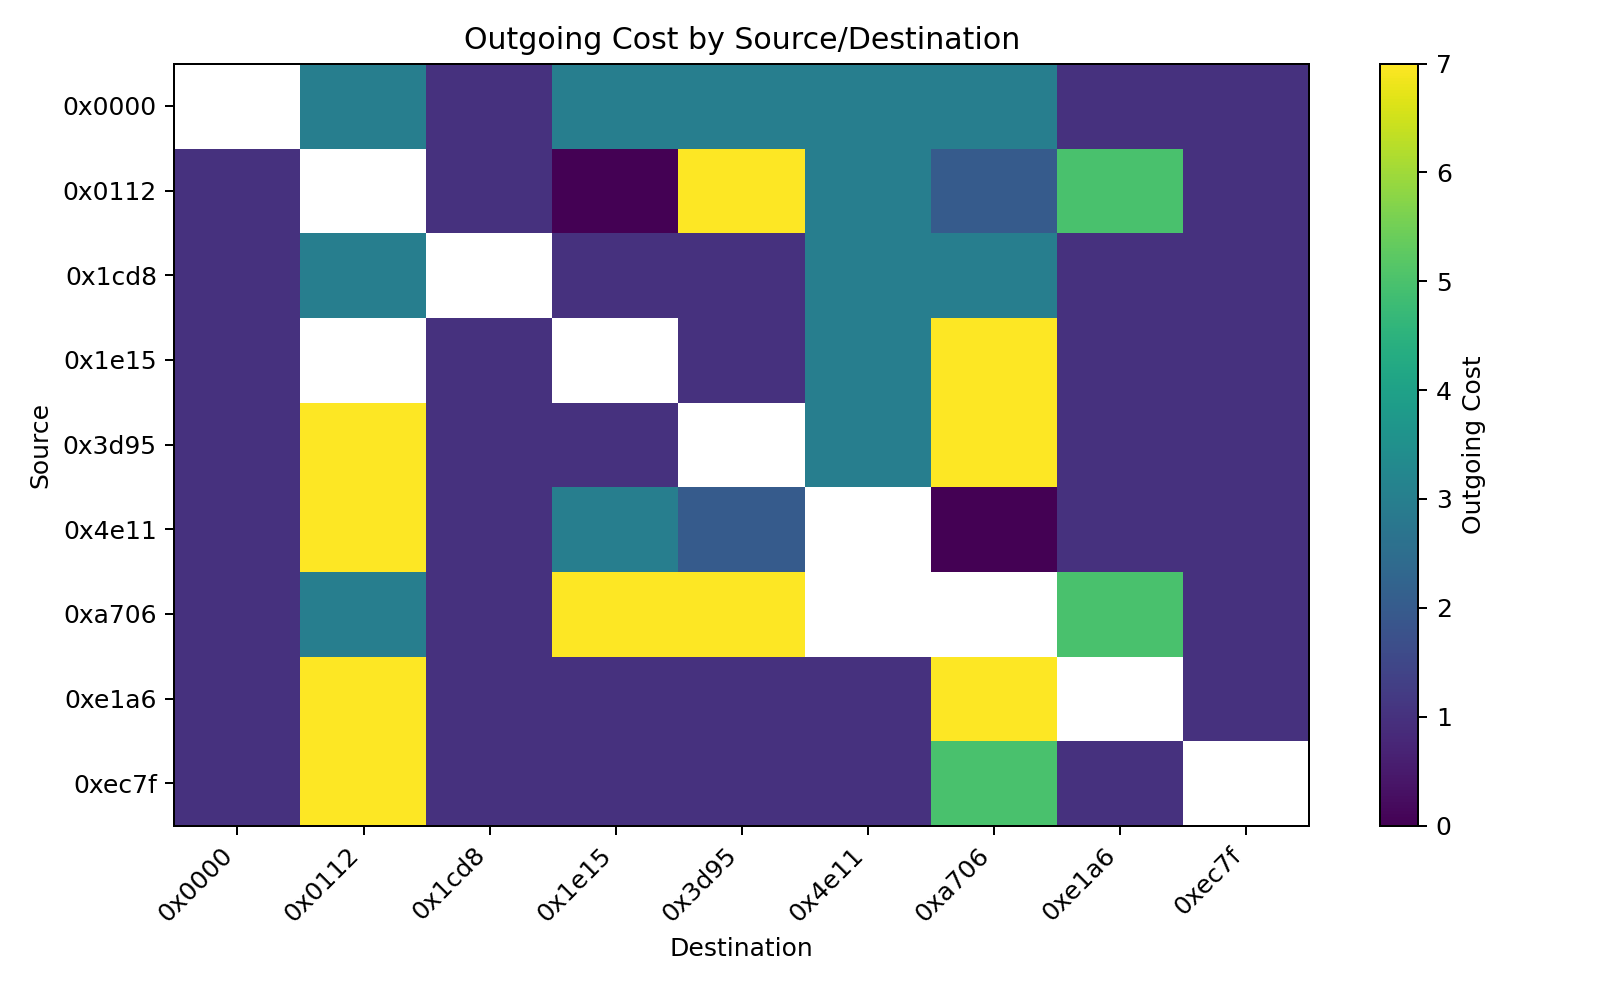
\includegraphics[width=0.86\linewidth]{report_assets/outgoing_cost_heatmap.png}
\caption{Outgoing cost matrix generated from \texttt{outgoing\_cost.csv}.}
\end{figure}

\section*{ThingSpeak Branch}

The ThingSpeak branch starts after the 200 received ID messages have been
processed. The function \texttt{prepare ThingSpeak messages} reads the final
Link Status state from the flow variables, then:

\begin{enumerate}
    \item finds the smallest source address, interpreting addresses as
    hexadecimal numbers;
    \item selects the destinations associated with that source;
    \item sorts those destinations in ascending hexadecimal order;
    \item sends each outgoing cost to ThingSpeak in \texttt{field1}.
\end{enumerate}

The HTTP request URL is built as:
\begin{center}
  \texttt{https://api.thingspeak.com/update?api\_key=WRITE\_API\_KEY\&field1=VALUE}.
\end{center}

The API key is read from the environment variable
\texttt{THINGSPEAK\_WRITE\_API\_KEY}. It is not stored inside
\texttt{flows.json}. The \texttt{ThingSpeak 1 msg / 20s} delay node is
configured in queue mode and enforces one update every 20 seconds.

The public ThingSpeak channel used for the submission is:
\begin{center}
  \texttt{https://thingspeak.mathworks.com/channels/3368448}
\end{center}
The channel identifier is \texttt{3368448}.

\begin{figure}[H]
\centering
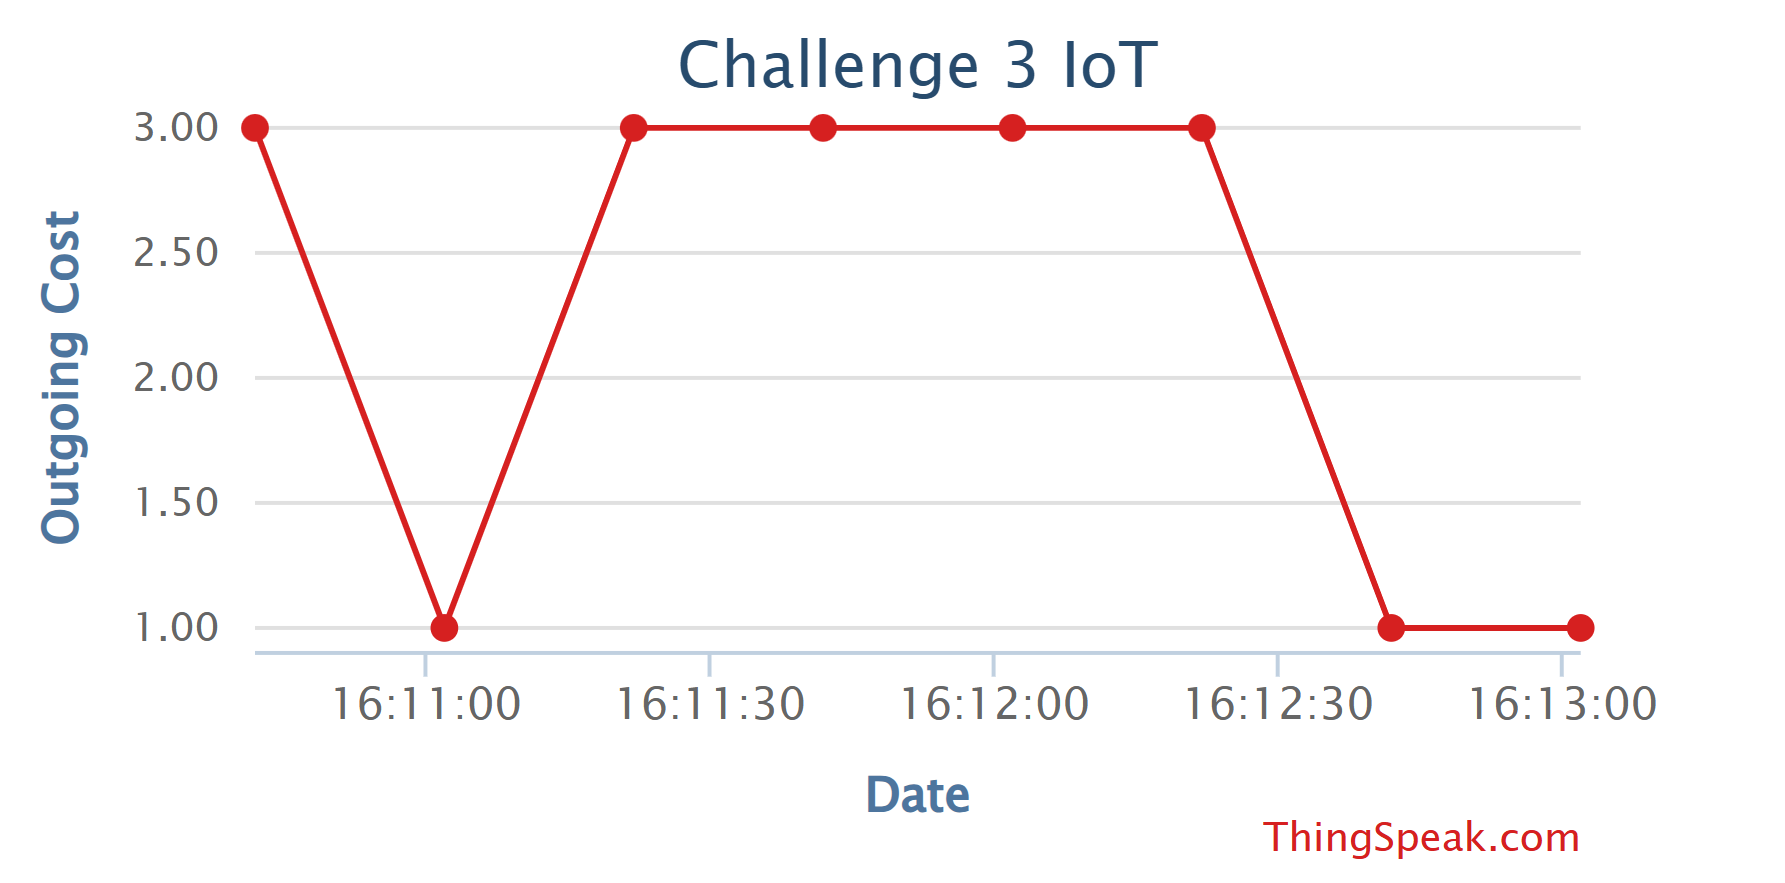
\includegraphics[width=0.86\linewidth]{report_assets/image.png}
\caption{ ThingSpeak chart for field1 outgoing cost updates.}
\end{figure}


\section*{Produced Deliverables}

The Node-RED execution produces the following CSV files:

\begin{itemize}
    \item \texttt{id\_log.csv}, containing the generated ID messages;
    \item \texttt{filtered\_elems.csv}, containing complete filtered attributes;
    \item \texttt{outgoing\_cost.csv}, containing the final outgoing cost for
    each processed source/destination pair while preserving processing order.
\end{itemize}

The Node-RED flow is exported as JSON and delivered as \texttt{nodered.txt}.

\end{document}
